\begin{frame}
  \begin{textblock*}{50mm}[1,1](61mm,195mm)
    
\includegraphics[height=4\baselineskip]{img/pseudo_logo_CSIRL.pdf}
  \end{textblock*}

  \begin{textblock*}{7cm}[0,1](67.6mm,190mm)
    \vbox{\structure{\LARGE CS IRL}

    \medskip
    {\large Computer Science In Real Life}}
  \end{textblock*}


  \begin{center}
    \structure{\Huge Les algorithmes}

    \bigskip
    \bigskip
    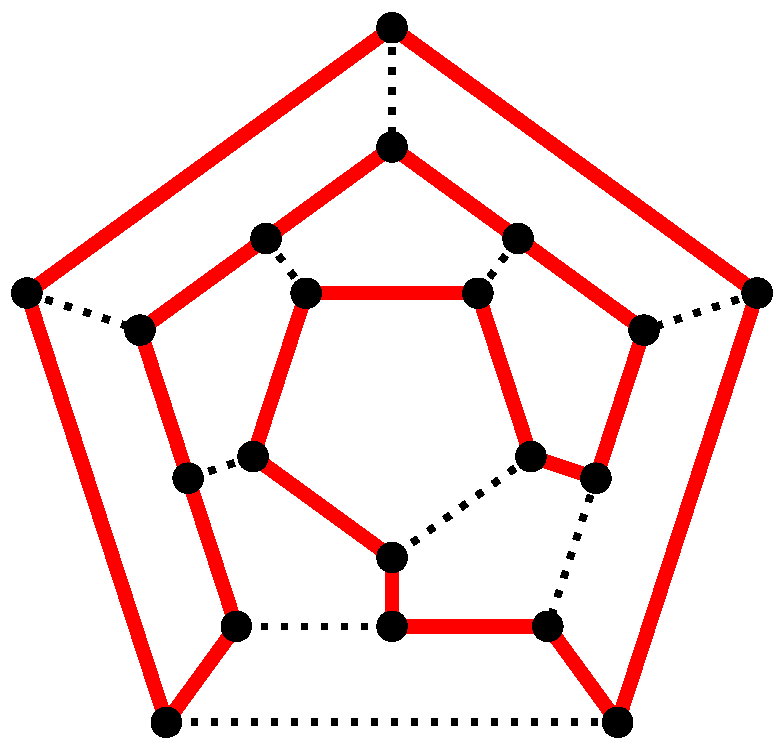
\includegraphics[width=.7\linewidth]{img/Hamiltonian_path.pdf}\label{img:hamiltonian}
    \vspace{5\baselineskip}


    ~

  \end{center}

  
\end{frame}

\begin{frame}
  \vspace{15\baselineskip}
  \vfill
  \begin{block}{À propos de ce document}
    \begin{itemize}
    \item \copyright\ 2011-2012 membres du projet CS IRL. Tous droits réservés.

    \item CS IRL est un \alert{projet libre et ouvert}: vous pouvez copier et
      modifier librement les ressources de ce projet sous les conditions
      données par la CC-BY-SA (en bref, vous pouvez diffuser et modifier ces
      ressources à condition que vous donniez les mêmes droits aux utilisateurs
      de vos copies).
    \item La page web du projet est ici: \url{http://www.loria.fr/~quinson/Mediation/CSIRL/}
    \item Les sources des ressources du projet sont entre autres ici: \url{http://github.com/jcb/CSIRL}
    \item Si vous le souhaitez, vous pouvez nous joindre ici: \url{discussions@listes.nybi.cc}
    \end{itemize}
  \end{block}

  \begin{block}{\normalsize Crédits image}\footnotesize
    P\pageref{img:hamiltonian}: Chemin hamiltonien par Ch. Sommer (licence GFDL/CC-BY-SA)
    \url{http://en.wikipedia.org/wiki/File:Hamiltonian_path.svg}

    P\pageref{img:CSmajor}: Computer Science Major (licence CC-BY-NC)
    \url{http://abstrusegoose.com/206}

%    P\pageref{img:realprog}: Real programmers: \alert{Dessin non libre, à refaire.}
%    \url{http://www.ninisworld.com/oddsends/justforfun/50realprogrammers.html}

    P\pageref{img:tsp}: exemple de TSP adapté de Wikipedia (licence GFDL/CC-BY-SA)
    \url{http://en.wikipedia.org/wiki/File:Aco_TSP.svg}
    
    P\pageref{img:tsp_xkcd}: Travelling Salesman Problem par XKCD (licence CC BY-NC 2.5)
    \url{http://xkcd.com/399/}

  \end{block}
\end{frame}
%%%%%%%%%%%%%%%%%%%%%%%%%%%%%%%%%%%%%%%%%%%%%%%%%%%%%%%%%%%%%%%%%%%%%%%%%%%%%%%%%%%%%%%%
\begin{frame}{Computer Science IRL -- Informatique sans ordinateur\\[-5pt]
  {\large Présentation du projet}}

% Contrairement à ce que beaucoup de monde pense, les ordinateurs ne sont pas la
% seule raison d'être de l'informatique. Pour preuve, ce projet développe
% diverses activités à faire avec des pions, des jetons ou des bouts de bois,
% mais sans aucun ordinateur et même sans électricité. Pourtant, ces petits jeux
% permettront à chacun de découvrir de manière ludique les notions au cœur de
% l'informatique: ce qu'est un algorithme et qu'est ce qui fait qu'un algorithme
% est meilleur qu'un autre, ou encore comment coder et transmettre une
% information.


  \begin{block}{CS IRL? Qu'est ce que c'est?}
    \begin{itemize}
    \item Des activités présentant les bases de l'informatique, mais sans
      ordinateur
    \item Pour chaque activité, un support matériel est proposé pour permettre
      d'\textit{apprendre avec les mains}
    \item Les activités sont rangées en séances cohérentes et progressives
%    \item C'est un projet libre, que vous pouvez télécharger, améliorer et
%      diffuser librement
    \item[
\includegraphics{img/rightpointing_magnifying_glass.pdf}]
      Computer Science In Real Life: Computer Science est la science
      informatique en anglais, tandis que IRL est l'abréviation utilisée sur
      internet pour décrire la vraie vie, ce qui n'est pas sur internet.
    \end{itemize}
  \end{block}

  \begin{block}{Les séances existantes dans la série}
    \begin{itemize}
    \item \structure{Les algorithmes:} Qu'est ce qu'un algorithme? Et une
      heuristique? À quoi ça sert?
    \item \structure{Codes et représentations:} Comment les ordinateurs codent
      et manipulent les données \textit{(à venir)}
    \item \structure{Turzzle:} puzzle de programmation sans ordinateur 
      \textit{(à venir)}
    \end{itemize}
  \end{block}
  \vspace{2\baselineskip}

  \begin{block}{Objectif de la séance algorithmique}
    \begin{itemize}
    \item Expliquer ce qu'est un algorithme et à quoi ça sert quand on veut
      utiliser un ordinateur
    \item Montrer un aspect du travail d'un informaticien, et de celui d'un
      chercheur en informatique
    \item La durée envisagée est d'une heure et demi ou deux heures.
    \item Ce n'est donc pas un cours complet sur l'algorithmique, qui nécessite
      25 à 50h au minimum.\\
      Cours pour aller plus loin (en 48h):
      \url{http://www.loria.fr/~quinson/Teaching/TOP/}
    \item[
\includegraphics{img/rightpointing_magnifying_glass.pdf}]
      Si vous êtes l'animateur, vous trouverez des conseils et des astuces dans le coin de l'animateur en page~\pageref{coin::animateur}.
    \end{itemize}
  \end{block}

  \begin{block}{Matériel nécessaire pour cette séance}
    \begin{itemize}
    \item Des clous, dont un coloré
    \item Des petites planches de tailles différentes
    \item Des legos: cinq couleurs, avec à chaque fois deux pièces $2\times2$ et une
      pièce $4\times2$
    \item Une planche avec des clous plantés (mais qui dépassent); Une cordelette et un marqueur
    \end{itemize}
  \end{block}
\end{frame}
%%%%%%%%%%%%%%%%%%%%%%%%%%%%%%%%%%%%%%%%%%%%%%%%%%%%%%%%%%%%%%%%%%%%%%%%%%%%%%%%%%%%%%%%%%
\begin{frame}{Computer Science IRL -- La séance algorithmique}
  \begin{block}{Introduction: les principales caractéristiques d'un ordinateur}
    \begin{itemize}
    \item \structure{Il est très \alert{rapide}:} il peut calculer de 1 à 1
      million en moins d'une seconde
    \item \structure{Il est parfaitement \alert{obéissant}:} il fait
    tout le temps exactement ce qu'on lui demande
    \item \structure{Il est absolument \alert{stupide}:} il exécute les
      ordres qu'on lui donne, sans la moindre capacité d'initiative.
      \begin{itemize}
      \item Par exemple, si on demande à un ordinateur de s'arrêter, il le fait\ldots
      \item Autre exemple, quand j'indique à des amis comment venir chez moi,
        je leur donne des indications comme "troisième à droite" ou "à gauche
        au 2ieme feu". Si je me trompe dans mes indications ("à gauche" au lieu
        de "à droite") et que cela les ferait prendre l'autoroute à
        contre-sens, mes amis vont faire preuve de sens commun et ne pas
        appliquer la consigne. Les ordinateurs n'ont \textbf{aucun} sens commun.
      \item Bug (n.m.): consigne erronée donnée par un humain et appliquée bêtement par une machine.

      \end{itemize}

    \end{itemize}
  \end{block}\vspace{-.5\baselineskip}

  \begin{block}{Le travail d'un informaticien}
    \begin{itemize}
    \item Se faire obéir d'un serviteur aussi stupide qu'un tas de fil demande
      un peu d'organisation
    \item Pour décomposer suffisamment les tâches à réaliser, il réfléchit à
      \textbf{comment} faire\\
      {\small (un peu comme un cycliste qui descendrait du vélo pour se regarder
        pédaler afin d'expliquer ensuite comment faire)}
    \item Pour chaque problème, il faut d'abord définir:
      \begin{itemize}
      \item \structure{la situation initiale:} le point de départ du problème
      \item \structure{les opérations possibles:} ce que j'ai le droit de faire pour faire
        évoluer la situation
      \item \structure{la situation finale:} ce vers quoi je veux tendre, l'état
        du problème quand je l'ai résolu
      \end{itemize}
    \end{itemize}
  \end{block}

  \centerline{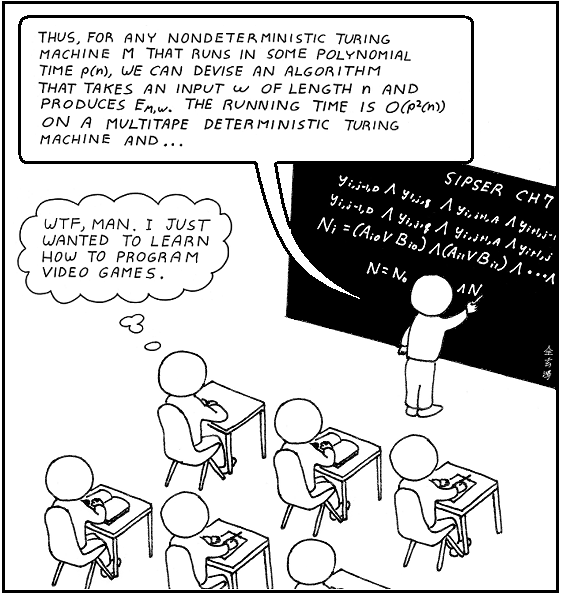
\includegraphics[width=.4\linewidth]{img/computer_science_major.PNG}\label{img:CSmajor}}
\end{frame}

%%% Local Variables: 
%%% mode: latex
%%% TeX-master: "CSIRL"
%%% End: 
